\documentclass{article}
\usepackage{graphicx}
\usepackage[margin=1.5cm]{geometry}
\usepackage{amsmath}

\begin{document}

\title{Warm-Up 16}
\author{Prof. Jordan C. Hanson}

\maketitle

\section{Confidence Intervals, Confidence Levels}

\begin{enumerate}
\item Consider Fig. \ref{fig:higgs}.  This is a graph of the number of times the CMS detector at the Large Hadron Collider detected subatomic particles with energy plotted on the x-axis.  Scientists were searching for the Higgs boson, a subatomic particle thought to control the mass of all the other particles.  In the graph, we see black data points, which are a histogram.  The errorbars in the y-direction represent the standard deviation in the mean for the individual data point.  Notice the \textit{bump} near $x = 125$.  (a) About how many standard deviations above the ``background'' prediction is teh data point? (Estimate). (b) What is the probability that the central black data point that is farthest from ``background'' occurred randomly (Estimate based on your answer in part (a)). (c) At what confidence level can you say the black data points in the bump did \textit{not} occur randomly?  (The green and yellow bands represent the 1 and 2 sigma confidence intervals for background).
\begin{figure}[ht]
\centering
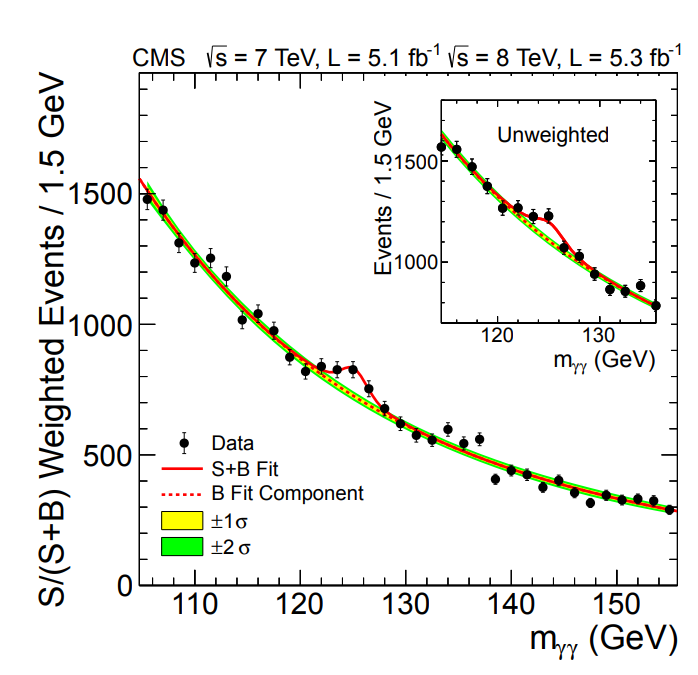
\includegraphics[width=0.5\textwidth]{higgs.png}
\caption{\label{fig:higgs} The number of ``events'' (hits) in the CMS detector at the Large Hadron Collider, versus particle energy, for a particularly special type of particle.  The green and yellow bands represent the 68 and 95 percent confidence intervals \textit{versus energy} for \textbf{background events.}  Background events do not represent the discovery of a brand new subatomic particle.}
\end{figure}
\end{enumerate}

\end{document}